\section{Center of Mass}

\blue{Take from the TAM 212 reference page - Centers of Mass - Introduction section}

%Lectures 28, 29 

\subsection{Basis Shapes}

\blue{Take from the TAM 212 reference page - Centers of Mass - Simplified Shapes}

Centroids of simple shapes can be combined to solve for the centroid of more complex parts. 

\subsection{Centroid}

The centroid denotes the \textit{geometric} center of an object. When an object is made of a homogeneous material, the centroid and the center of mass are at the same point. If the object has an axis of symmetry, the centroid is on the axis of symmetry. In some cases, the centroid may not be on the object. 

\blue{Should we include an example problem from lecture 28?}

\begin{figure*}[!h]
\centering
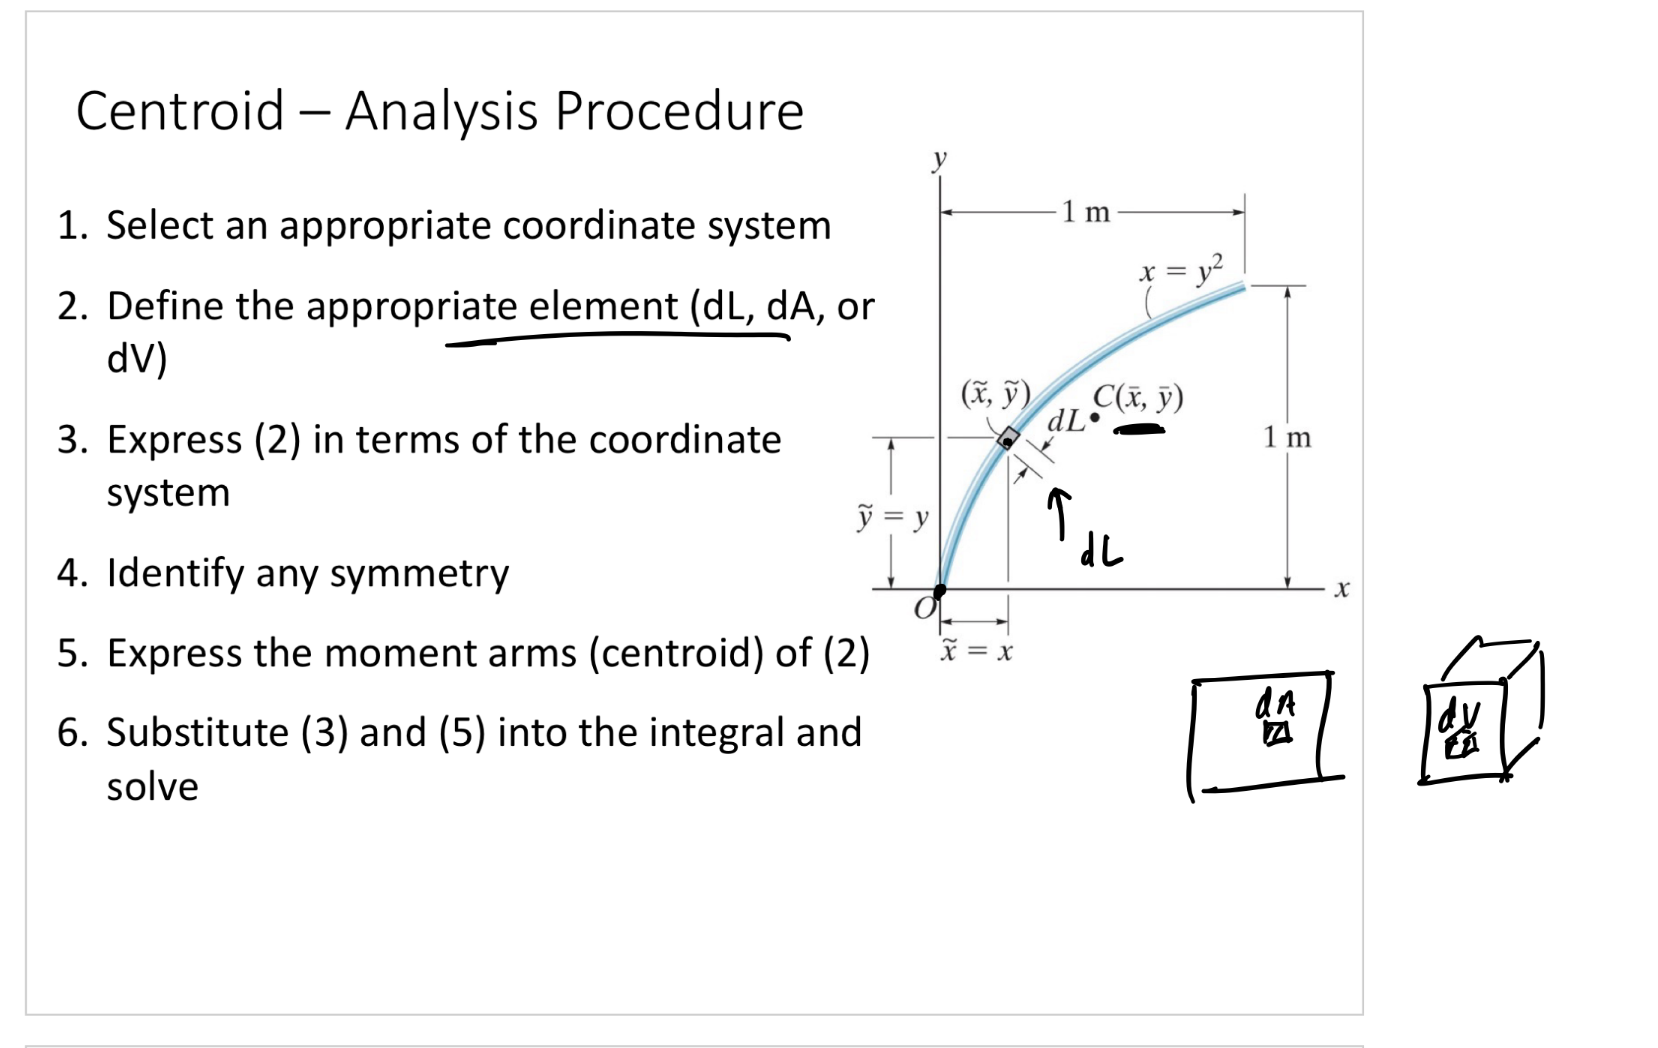
\includegraphics[angle=0, width=5 in]{COMFigures/CentroidAnalysis.png}
\vspace{-2mm}
\caption{\small Nonuniform load. Need to remake this in the same style as the other pictures.}
\vspace{-3mm}
\label{Fig:CentroidAnalysis}
\end{figure*}

